\documentclass[en]{../../../../../../eplexam}
\usepackage{circuitikz}

\hypertitle{sigsys-FSAB1106}{4}{FSAB}{1106}{2012}{Juin}
{Louis Devillez}
{Luc Vandendorpe et Vincent Wertz}


\section{Question 1: LV1}
Considérons le filtre RLC passif de la \textsc{Figure \ref{RLC}}. On s'intéresse à la relation qu'il y a entre tension de source x(t) et la tension aux bornes de l'inductance L, notée $y(t) = v_L(t)$

Pour rappel, les courants $i_C(t)$ et $i_L(t)$ dans la capacité C et l'inductance L sont respectivement donnés par:
$$i_C(t) = C \cfrac{dv_C(t)}{dt} $$
$$v_L(t) = L \cfrac{di_L(t)}{dt}$$
où $v_C(t)$ et $v_L(t)$ désignent les tensions aux bornes de la capacité et de l'inductance.
\begin{figure}[!ht]
	\centering
	\begin{circuitikz}[american]
		\draw (0,0) to[V=x(t)] (0,2) to[R] (2,2) to [L](4,2) to[C] (4,0) --(0,0);
	\end{circuitikz}
	\caption{Filtre RLC série}
	\label{RLC}
\end{figure}
L'équation différentielle qui lie x(t) et y(t) est donnée par
$$LC \frac{d^{2}y(t)}{dt^{2}}+RC\frac{dy(t)}{dt}+ y =LC\frac{d^2x(t)}{dt^2}$$
\begin{itemize}
	\item Calculez la réponse en fréquence du système
	\item Calculer la réponse impulsionnelle de ce système pour le jeu de paramètre suivants: $L = 0.5 mH$, $C=100\mu F$ et $H = 15\Omega$
	\item Dessinez le diagramme de bode de ce système (module UNIQUEMENT de la fonction de transfert) pour les même paramètres
	\item Si l'on introduit dans le système un signal d'entrée donné par $x(t) = \cos(\omega_0t+\phi_0) +0.1\sin(\omega_1t + \phi_1)$, qu'obtient-on comme signal de sortie, y(t)?
\end{itemize}

\begin{solution}
	\begin{itemize}
		\item Fonction de transfert 
		$$H(jw) = \cfrac{LC(j\omega)^2}{LC(j\omega)^2+RC(j\omega)+1} $$
		\item Réponse impulsionnelle 
		$$H(jw) = \cfrac{0.5*10^{-6}(j\omega)^2}{0.5*10^{-6}(j\omega)^2+15*10^{-4}(j\omega)+1} = 1 - \frac{-3000j\omega - 2*10^6}{(j\omega+2000)(j\omega+1000)} $$
		$$H(j\omega) = 1 - \frac{4000}{j\omega + 2000} + \frac{1000}{j\omega +1000} $$
		$$y(t) = \delta(t)  + (1000e^{-1000t}- 4000e^{-2000t})u(t)$$
		
		\item diagramme de bode 
		$$H(jw) = \cfrac{(j\omega)^2}{(j\omega+2000)(j\omega+1000)} = \cfrac{(j\omega / \sqrt{2}*10^3)^2}{(j\omega/2*10^3+1)(j\omega/10^3+1)}  $$
		\begin{center}		
			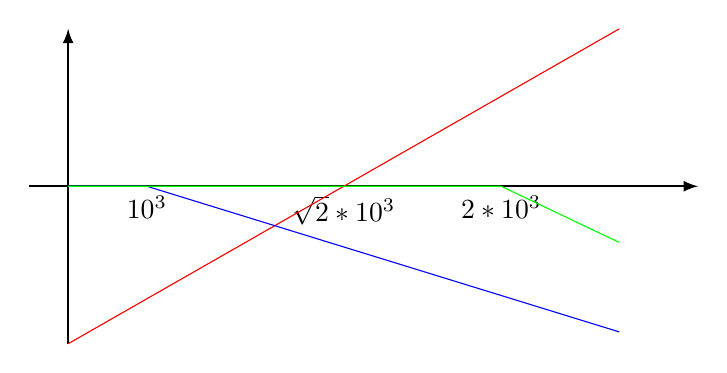
\begin{tikzpicture}
			\draw [thick,-latex] (-0.5,0) -- (8,0);
			\draw [thick,-latex] (0,-2) -- (0,2);
			\draw (1,0)node[below]{$10^3$};
			\draw (3.5,0)node[below]{$\sqrt{2}*10^3$};
			\draw (5.5,0)node[below]{$2*10^3$};
			\draw [red] (0,-2)--(7,2);
			\draw [blue] (0,0) -- (1,0) -- (7,-1.85);
			\draw [green] (0,0) -- (5.5,0) -- (7,-0.714);
			\end{tikzpicture} 
			
			\begin{tikzpicture}
			\draw [thick,-latex] (-0.5,0) -- (8,0);
			\draw [thick,-latex] (0,-2) -- (0,2);
			\draw (1,0)node[below]{$10^3$};
			\draw (3.5,0)node[below]{$\sqrt{2}*10^3$};
			\draw (5.5,0)node[below]{$2*10^3$};
			\draw [red] (0,-2)--(1,-1.42) -- (5.5,-0.19) -- (7,-0.19);
			\end{tikzpicture}
		\end{center}
	\end{itemize}
	
	\item
	$$y(t) =|H(j\omega_0)| \cos(\omega_0t+\phi_0 + \theta_0) +|H(j\omega_1)|0.1\sin(\omega_1t + \phi_1 + \theta_1)$$
	avec:
	\subitem$\theta_0 = angle(|H(j\omega_0)|)$
	\subitem $\theta_1 = angle(|H(j\omega_1)|)$
\end{solution}

\section{Question 2: LV2}
On s'intéresse à un système linéaire permanent fonctionnant en temps discret. Lorsqu'on lui entre le signal $x\left[n\right]$ donné à la \textsc{Figure \ref{signal}}, il en sort le signal $y\left[n\right]$ donné par la même figure.
\begin{figure}[!ht]
	\centering
	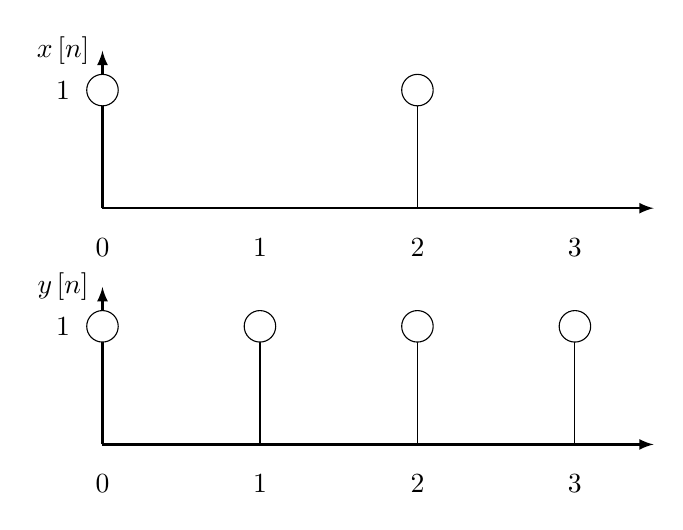
\begin{tikzpicture}
		\draw [thick,-latex] (0,0) -- (0,2);
		\draw [thick,-latex] (0,0) -- (7,0);
		\foreach \r in {0,...,3}
		{
			\draw (\r*2,-0.5)node[]{\r};	
		}
		\draw (-0.5,2)node[]{$x\left[n\right]$};
		\draw (-0.5,1.5)node[]{1};
		\draw [fill =white] (0,1.5)circle(0.2);
		\draw (4,0) -- (4,1.5);
		\draw (4,1.5)[fill =white] circle(0.2);
		
		\draw [thick,-latex] (0,-3) -- (0,-1);
		\draw [thick,-latex] (0,-3) -- (7,-3);
		\foreach \r in{0,...,3}
		{
			\draw (\r*2,-3.5)node[]{\r};
			\draw (\r*2,-3) -- ++ (0,1.5);
			\draw (\r*2,-1.5) [fill =white] circle(0.2);	
		}
		\draw (-0.5,-1) node[]{$y\left[n\right]$};
		\draw (-0.5,-1.5)node[]{1};
	\end{tikzpicture}
	\caption{Signaux d'entrée et de sortie}
	\label{signal}
\end{figure}

\begin{itemize}
	\item Donnez la réponse impulsionnelle $h\left[n\right]$ de ce système. Une réponse rapide est possible mais doit être justifiée par une ou deux phrases.
	\item Donnez la réponse en fréquence $H(e^{j\omega})$ de ce système
	\item Si l'on introduit dans ce système un signal de type $\cos\left[n\omega_0\right]$, donnez l'expression du signal de sortie
\end{itemize}

\begin{solution}
	$$x\left[n\right] = \delta \left[0\right] + \delta \left[n-2\right]$$
	$$X(e^{j\Omega}) = 1 + e^{-2j\Omega} $$
	$$y\left[n\right] = \delta \left[0\right] + \delta \left[n-1\right]+ \delta \left[n-2\right]+ \delta \left[n-3\right]$$
	$$Y(e^{j\Omega}) = 1 + e^{-j\Omega} + e^{-2j\Omega} + e^{-3j\Omega} =(1+e^{-j\Omega})(1+e^{-2j\Omega}) $$
	$$H(e^{j\Omega}) = \cfrac{Y(e^{j\Omega})}{X(e^{j\Omega})} = 1+e^{-j\Omega} $$
	$$h\left[n\right] = \delta\left[n\right] + \delta\left[n-1\right]$$
	
	$$y(t) = \cos\left[n\omega_0\right]+\cos\left[(n-1)\omega_0\right]$$
\end{solution}

\section{Question 3: LV3}
On génère un signal périodique $x(t) = \cos(2\pi f_0 t)$. Ce signal est d'abord échantillonné par un échantillonneur qui fonctionne à cadence (fréquence) $f_e$. Ensuite le résultat de l'échantillonnage est interpolé par 2 filtres réels différents, fonctionnant en temps continu. L'un est de type passe-bas idéal et de fréquence de coupure $f_e/2$ (il laisse donc passe toutes les fréquences telles que $f<f_e/2$). Le deuxième filtre est un filtre passe-bande, et laisse passer toutes les fréquences $f$ telles $f_e/2 \le |f| \le f_e$. Le schéma complet est décrit à la \textsc{Figure \ref{filtre}}.

\begin{figure}[!ht]
	\centering
	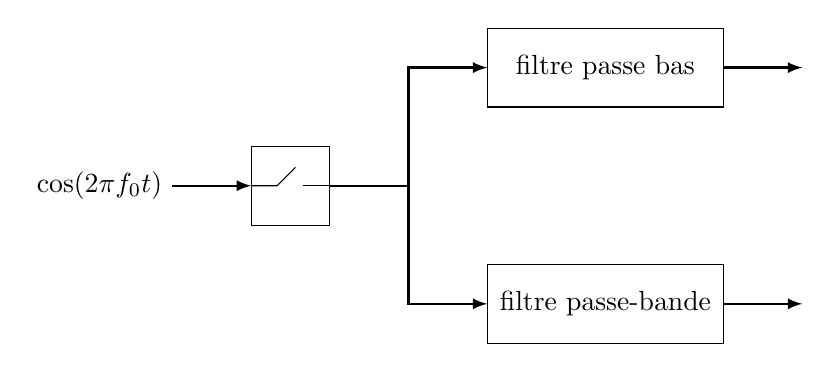
\begin{tikzpicture}
	\draw [thick,-latex] (0,0) node[left]{$\cos(2\pi f_0 t)$} -- (1,0);
	\draw (1,-0.5) rectangle (2,0.5);
	\draw (1,0) -- (1.33,0) -- ++(45:0.33);
	\draw (1.66,0) -- (2,0);
	\draw [thick,-latex] (2,0) -- (3,0) -- (3,1.5) -- (4,1.5);
	\draw [thick,-latex] (3,0) -- (3,-1.5) -- (4,-1.5);
	\draw (4,2) rectangle (7,1);
	\draw (4,-2) rectangle (7,-1) ;
	\draw (5.5,1.5) node[]{filtre passe bas};
	\draw (5.5,-1.5) node[]{filtre passe-bande};
	\draw [thick,-latex] (7,1.5) -- (8,1.5);
	\draw [thick,-latex] (7,-1.5) -- (8,-1.5);
	\end{tikzpicture}
	\caption{Séquence des opérations}
	\label{filtre}
\end{figure}

\begin{itemize}
	\item Représentez graphiquement le spectre du signal obtenu en sortie de chacun des 2 filtres analogiques lorsque $f_0 = f_e/4$ Expliquer.
	\item Représentez graphiquement le spectre du signal obtenu en sortie de chacun des 2 filtres analogiques lorsque $f_0 = 7f_e/8$ Expliquer.
	\item Représentez également graphiquement, et expliquer ce qui se passe en sortie de chacun de 2 filtres lorsque, à $f_e$ fixé, on augmente $f_0$ à partir de 0 jusque $3f_e/2$.
\end{itemize}

\begin{solution}
	\begin{itemize}
		\item Spectre du signal échantillonné $f_o = f_e/4$
		\begin{center}
			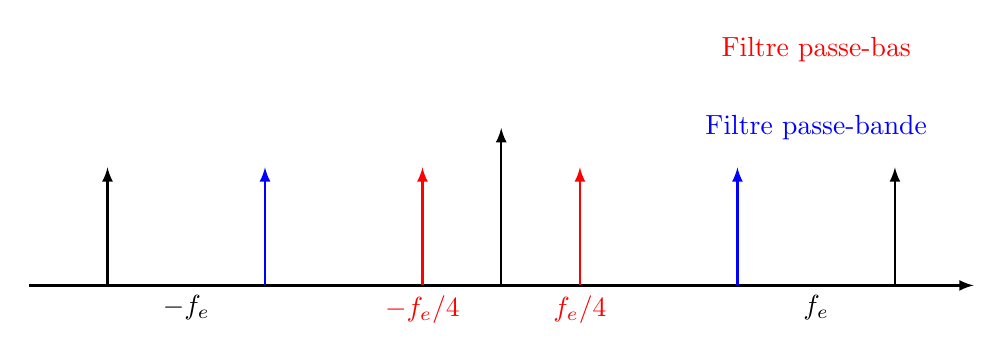
\begin{tikzpicture}
			\draw [thick,-latex](0,0) -- (0,2);
			\draw [thick,-latex] (-6,0) -- (6,0);
			\draw [thick,-latex,red] (1,0)node[below]{$f_e/4$} -- (1,1.5);
			\draw [thick,-latex,red] (-1,0)node[below]{$-f_e/4$} -- (-1,1.5);
			\draw [thick,-latex,blue] (3,0) -- (3,1.5);
			\draw [thick,-latex] (5,0) -- (5,1.5);
			\draw [thick,-latex,blue] (-3,0) -- (-3,1.5);
			\draw [thick,-latex] (-5,0) -- (-5,1.5);
			\draw (4,0)node[below]{$f_e$};
			\draw (-4,0) node[below]{$-f_e$};
			\draw (4,2)node[blue]{Filtre passe-bande};
			\draw (4,3)node[red]{Filtre passe-bas};
			\end{tikzpicture}
		\end{center}
		ici le théorème de Shannon est respecté le filtre passe bas nous donne bien notre signal de départ
		\item Spectre du signal échantillonné $f_o = 7f_e/8$
		\begin{center}
			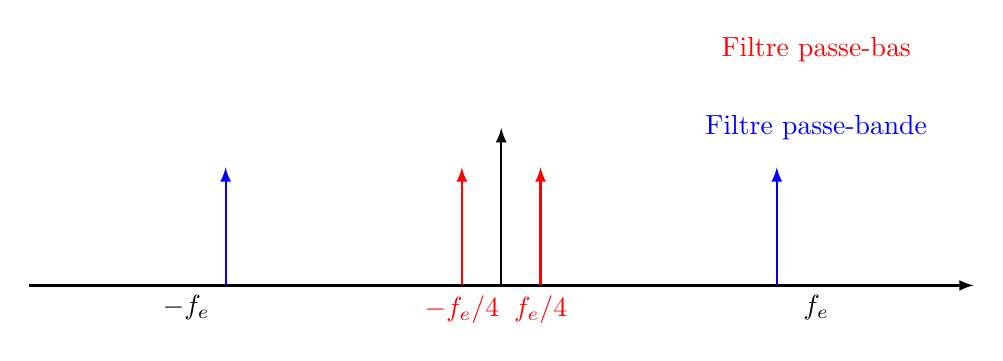
\begin{tikzpicture}
			\draw [thick,-latex](0,0) -- (0,2);
			\draw [thick,-latex] (-6,0) -- (6,0);
			\draw [thick,-latex,red] (0.5,0)node[below]{$f_e/4$} -- (0.5,1.5);
			\draw [thick,-latex,red] (-0.5,0)node[below]{$-f_e/4$} -- (-0.5,1.5);
			\draw [thick,-latex,blue] (3.5,0) -- (3.5,1.5);
			\draw [thick,-latex,blue] (-3.5,0) -- (-3.5,1.5);
			\draw (4,0)node[below]{$f_e$};
			\draw (-4,0) node[below]{$-f_e$};
			\draw (4,2)node[blue]{Filtre passe-bande};
			\draw (4,3)node[red]{Filtre passe-bas};
			\end{tikzpicture}
		\end{center}
		ici le théorème de Shannon n'est pas respecté le filtre passe bas ne nous donne pas le bon signal mais le filtre passe bande oui		
				
		\item
		\subitem $|f| < f_e/2$ le filtre passe bas renvoi le bon spectre et la fréquence renvoyée augmente avec f. Le filtre passe bande ne renvoi pas le bon spectre et la fréquence renvoyée diminue avec f
		
		\subitem $f_e < |f| < f_e$ le filtre passe bas ne renvoi pas le bon spectre et la fréquence renvoyée diminue avec f. Le filtre passe bande renvoi le bon spectre et la fréquence renvoyée augmente avec f.
		
		\subitem $|f| < f_e/2$ le filtre passe bas ne renvoi pas le bon spectre et la fréquence renvoyée augmente avec f. Le filtre passe bande ne renvoi pas le bon spectre et la fréquence renvoyée diminue avec f
	\end{itemize}
\end{solution}

\section{Question 3: VW1}
On considère un système LTI continu pour lequel la relation entre l'entrée x(t) et la sortie y(t) est donnée par
$$y''(t) - y'(t) -2y(t) = x(t) -x'(t)$$
\begin{itemize}
	\item Calculer la fonction de transfert H(s)
	\item Détermire la réponse impulsionnelle h(t) dans chacun des trois cas suivants:
	\subitem le système est causale
	\subitem le système est stable
	\subitem le système n'est ni causal ni stable
	\item D'autre cas sont-ils à envisager ?
	\item Explique brièvement la notion de système causal
\end{itemize}

\begin{solution}
	\begin{itemize}
		\item Fonction de transfert
		$$H(s) = \cfrac{1-s}{s^2-s-2} $$
		\item Réponse impulsionnelle
		$$H(s) = \cfrac{1-s}{(s-2)(s+1)} = \cfrac{-1/3}{s-2} + \cfrac{-2/3}{s+1}$$
		\subitem système causale
		$$h(t) = (-1/3e^{2t}-2/3e^{-t})u(t) $$
		\subitem le système est stable
		$$h(t) = 1/3e^{2t}u(-t)-2/3e^{-t}u(t) $$
		\subitem le système n'est ni stable ni causale
		$$h(t) = (1/3e^{2t}+2/3e^{-t})u(-t) $$
		
		\item avec 2 pôles il n'y a que 3 cas a envisager
		
		\item Un système est causale est un système tel que la  sortie dépend des valeurs passées et présentes
	\end{itemize}
	
	
\end{solution}

\section{Question 4:VW2}
On considère le système représenté par le schéma bloc suivant:
\begin{center}
	\begin{tikzpicture}
		\draw [thick,-latex](0,0)node[left]{x} -- (0.8,0);
		\draw (0.7,0)node[above]{+};
		\draw (1,0) circle(0.2);
		\draw [thick,-latex] (1.2,0) -- (2,0);
		\draw (2,0.5) rectangle (3.5,-0.5);
		\draw (4.5,0.5) rectangle (6,-0.5);
		\draw[thick,-latex] (3.5,0) -- (4.5,0);
		\draw (2.75,0)node[]{$\cfrac{1}{z-1/4}$};
		\draw (5.25,0)node[]{$\cfrac{1}{z-1/2}$};
		\draw [thick,-latex](6,0) -- (6.5,0) -- (6.5,-1.5) -- (4,-1.5);
		\draw (4,-2) rectangle (2.5,-1);
		\draw (3.25,-1.5)node[]{$-71/64$};
		\draw [thick,-latex](2.5,-1.5) -- (1.2,-1.5);
		\draw (1.3,-1.5) node[below]{+};
		\draw (1,-1.5) circle(0.2);
		\draw [thick,-latex] (1,-1.3) -- (1,-0.2);
		\draw (1,-0.3) node[left]{-};
		\draw[thick,-latex] (6.5,0) --(7.5,0);
		\draw (7.5,-0.5) rectangle (8.5,0.5);
		\draw (8,0)node[]{$\cfrac{1}{z}$};
		\draw [thick,-latex] (8.5,0) -- (9.3,0);
		\draw (9.2,0) node[above]{+};
		\draw (9.5,0)circle(0.2);
		\draw [thick,-latex] (6.5,0) -- (6.5,1) -- (9.5,1) -- (9.5,0.2);
		\draw (9.5,0.3)node[right]{+};
		\draw [thick,-latex] (9.7,0) -- (10.7,0)node[right]{y};
		\draw [thick,-latex] (9,0) -- (9,-3) -- (6,-3);
		\draw (6,-2.5) rectangle (4.5,-3.5);
		\draw (5.25,-3)node[]{$49/64$};	
		\draw [thick,-latex] (4.5,-3) -- (1,-3) -- (1,-1.7);
		\draw (1,-1.8) node[left]{+};	
	\end{tikzpicture}
\end{center}
\begin{itemize}
	\item Donner une représentation d'état de ce système
	\item Calculer la fonction de transfert de x vers y
	\item Étudier la stabilité interne du système
	\item Étudier la stabilité BIBO du système
	\item Sans calcul supplémentaire, que peut-on dire à propos de commandabilité et/ou d'observabilité ? Faire les calculs nécessaire pour vérifier cette affirmation
\end{itemize}

\begin{solution}
	\begin{itemize}
		\item Représentation d'état:	$$
		\begin{bmatrix}
		q_1\left[n-1\right]\\
		q_2\left[n-1\right]\\
		q_3\left[n-1\right] 
		\end{bmatrix}=
		\begin{bmatrix}
		1/4&71/64&-49/64\\
		1&1/2&0\\
		0&1&0
		\end{bmatrix}
		\begin{bmatrix}
		q_1\left[n\right]\\
		q_2\left[n\right]\\
		q_3\left[n\right] 
		\end{bmatrix}
		+
		\begin{bmatrix}
		1\\
		0\\
		0
		\end{bmatrix}
		x\left[n\right]$$
		$$
		y\left[n\right]=
		\begin{bmatrix}
		0 & 1&1
		\end{bmatrix}
		\begin{bmatrix}
		q_1\left[n\right]\\
		q_2\left[n\right]\\
		q_3\left[n\right] 
		\end{bmatrix}
		+
		\begin{bmatrix}
		0
		\end{bmatrix}
		x\left[n\right]$$
		
		\item Fonction de transfert
		$$H(z) = \cfrac{z+1}{(z+1)(z-7/8)^2}$$
		
		\item $|\lambda_i| \le 1$ le système est marginalement stable
		
		\item $|\lambda_i| < 1$ le système est BIBO stable
		
		\item puisque qu'il y a une simplification pôles zéros il y a une perte de commandabilité et/ou d'observabilité
		
		$$C= \begin{bmatrix}
		B\\
		AB\\
		A^2B
		\end{bmatrix} = 
		\begin{bmatrix}
		0&0&1\\
		0&1&\\
		1&1/4&
		\end{bmatrix}$$
		Le système est complètement commandable 
		$$O= \begin{bmatrix}
		C&CA&CA^2
		\end{bmatrix} = 
		\begin{bmatrix}
		1&1&0\\
		0&3/2&1\\
		49/64&119/64&7/4
		\end{bmatrix}$$
		$$det = 21/8-119/6449/64 = 0$$
		le système n'est pas complètement observable
	\end{itemize}
\end{solution}
\end{document}
